\chapter{Implementierung}
Nochmal die Forschungsfrage formulieren\\
Wie kann sich mit dem RFU6 über node opcua vebunden werden und auf dessen Methoden zugegriefen werden?


\section{Abfragen der Ids}
Um Methoden aufzurufen werden die jeweiligen NodeIds der verschiedenen Knoten benötiegt. 

OPC UA verwendet Namespaces, um eindeutige Kennungen über verschiedene Namensbehörden hinweg zu erstellen, die OPC UA-Informationmodelle definieren.\\

Die Attribute NodeId und BrowseName sind Kennungen eines Knotens. Ein Knoten im OPC UA-Adressraum wird eindeutig durch eine NodeId identifiziert. Im Gegensatz dazu kann der BrowseName nicht verwendet werden, um einen Knoten eindeutig zu identifizieren, da verschiedene Knoten denselben BrowseName haben können. Der BrowseName wird verwendet, um einen Pfad zwischen zwei Knoten zu erstellen oder eine Standard-Eigenschaft zu definieren.\\

Ein Namespace wird durch einen Namespace-URI identifiziert. Der URI ist der Bezeichner für ein OPC UA-Informationmodell, das von einer Arbeitsgruppe als Namensbehörde entwickelt wurde. Der URI für den Basis-OPC-UA-Namespace, der von der OPC-UA-Arbeitsgruppe definiert wurde, lautet \url{'http://opcfoundation.org/UA/'}.\\

Ein oder mehrere Instanz-Namespaces werden verwendet, um die serverspezifischen Instanzen von Standard- oder anbieterspezifischen Objekttypen bereitzustellen. Objektinstanzen sollten nicht mit Typknoten in einem Namespace gemischt werden, solange diese Typknoten in verschiedenen Servern wiederverwendet werden.\cite{.01.03.2021}\\

Sowohl die NodeId als auch der QualifiedName (DatenTyp für BrowseName) enthalten einen NamespaceIndex und eine Kennung. Der NamespaceIndex ist der Index in einer Namespace-Tabelle, die vom OPC UA-Server verwaltet wird. Die Namespace-Tabelle ist eine Eigenschaft, bei der der Wert ein Array von Zeichenfolgen ist. Jede Zeichenfolge ist ein Namespace-URI, der vom Server verwendet wird. Der Index in diesem Array ist der NamespaceIndex, der in NodeId und QualifiedName verwendet wird. Siehe auch OPC UA NodeId-Konzepte.\\

Um auf die Methoden des RFU6 zuzugreifen, werden die Namespace-Indizes der Node-IDs benötigt. Auch müssen die Ids für jeden Sitzung neue abgefragt werden da, sich die Ids verändern könnten.\\

Server dürfen den Namespace-Index für eine bestimmte Namespace-URI nicht ändern oder Einträge aus der Namespace-Tabelle löschen, solange eine aktive Sitzung besteht. So können Clients die Namespace-Tabelle für eine bestimmte Sitzung zwischenspeichern. Ein Server darf jedoch Namespace-Indizes ändern und Einträge aus der Namespace-Tabelle löschen, wenn kein Client verbunden ist oder wenn der Server neu gestartet wird. 
Aus diesem Grund sollte ein Client den Namespace-Index nicht speichern, ohne auch die Namespace-URI zu speichern, da eine Namespace-URI, die während einer Sitzung durch den Index \frqq  2 \flqq dargestellt wird, während der nächsten Sitzung durch den Index \frqq  5 \flqq dargestellt werden könnte. Daher sollte ein Client immer die Namespace-Tabelle des Servers lesen und die Namespace-Indizes aktualisieren, bevor er Dienste aufruft, bei denen NodeIds involviert sind, nachdem er eine Sitzung mit einem Server hergestellt hat.\\

Es gibt mehrere Möglichkeiten auf die NamespaceIndexe der NodeIds zuzugreifen.\\ 

Eine Möglichkeiten  ist die einen Addressraum zu erstellen und auf dessen Methode \frqq getNamespaceindex\flqq   auf die Id zuzugreifen.

Das Hauptziel des OPC UA-Adressraums ist es, eine standardisierte Möglichkeit für Server bereitzustellen, Objekte für Clients darzustellen. Das OPC UA-Objektmodell wurde entworfen, um dieses Ziel zu erreichen. Es definiert Objekte in Bezug auf Variablen und Methoden. Es ermöglicht auch die Darstellung von Beziehungen zu anderen Objekten.\cite{.11.04.2020}\\

\begin{lstlisting}[style=JavaScript, caption={Zugriff auf die Ids über den Addressraum}]
this.addressSpace = AddressSpace.create();
const namespace0 = this.addressSpace.getDefaultNamespace();

this.addressSpace.registerNamespace('http://opcfoundation.org/UA/AutoID/');
this.nsAutoID = this.addressSpace.getNamespaceIndex('http://opcfoundation.org/UA/AutoID/');
if (this.nsAutoID === -1) throw new Error(" cannot find AutoID namespace" );

this.addressSpace.registerNamespace(" http://opcfoundation.org/UA/DI/" );
this.nsOpcDI = this.addressSpace.getNamespaceIndex(" http://opcfoundation.org/UA/DI/" );

this.addressSpace.registerNamespace('http://www.sick.com/RFU6xx/');
this.nsRfu = this.addressSpace.getNamespaceIndex('http://www.sick.com/RFU6xx/');
\end{lstlisting}

In Zeile sechs wird eine Überprüfung auf minus eins durchgeführt. Wenn der Namespace zuvor nicht registriert ist, wird wird minus als Index zurückgegeben. Die Ids werde hier im Konstruktor abgefragt.\\

Die zweite Möglcihkeit ist es über die Session auf das Namespace Array zuzugreifen. Aus diesem Array werdem die NamespaceIndexe ausgelesen.\\

Der Index, den ein OPC UA-Server für eine Namespace-URI verwendet. Die Namespace-URI identifiziert die Namensautorität, die die Bezeichner von NodeIds definiert, z.B. die OPC Foundation, andere Standardisierungsgremien und Konsortien, das zugrunde liegende System oder den lokalen Server. Sie werden im sogenannten Namespace-Array (auch Namespace-Tabelle genannt) gespeichert. Namespace-Indizes sind numerische Werte, die zur Identifizierung von Namespaces zur Optimierung von Übertragung und Verarbeitung verwendet werden. Der Namespace-Index ist der Index der Namespace-URI im Namespace-Array.\\

\begin{lstlisting}[style=JavaScript, caption={Zugriff auf die Ids über die Session}]
async init(){		
    const nsArray = await this.session.readNamespaceArray();
    this.nsAutoId = this.session.getNamespaceIndex('http://opcfoundation.org/UA/AutoID/');
    this.nsOpcDI  = this.session.getNamespaceIndex(" http://opcfoundation.org/UA/DI/" );
    this.nsRfu    = this.session.getNamespaceIndex('http://www.sick.com/RFU6xx/');
}
\end{lstlisting}

Der Zugriff auf das Namespace-Array über die Session und damit auf die Methode \frqq readNamespaceArray()\flqq   hat den Nachteil, dass diese nicht im Konstruktor aufgerufen werden kann. Die Methode \frqq readNamespaceArray()\flqq   kann nicht im Konstruktor aufgerufen werden, da sie asynchron ist.\\

Asynchrone Funktionen können null oder mehrere await-Ausdrücke enthalten. Await-Ausdrücke bewirken, dass Promises-rückkehrende Funktionen sich so verhalten, als ob sie synchron wären, indem sie die Ausführung aussetzen, bis das zurückgegebene Promise erfüllt oder abgelehnt wird. Der aufgelöste Wert des Promise wird als Rückgabewert des await-Ausdrucks behandelt. Die Verwendung von async und await ermöglicht die Verwendung von gewöhnlichen try/catch-Blöcken um asynchronen Code.\\

Somit ist die Funktion \frqq async init()\flqq   erforderlich, da es nur innerhalb von async-Funktionen möglich ist, \frqq await\flqq   zu verwenden.\\

Der Zugriff auf NodeIds über den AddressSpace hat den Nachteil, dass er zwar positive Werte liefert, aber nicht mit den tatsächlichen NodeIds übereinstimmt, die mit dem UAExpert ausgelesen werden können.

Da durch fehlerhafte IDs das Aufrufen der Methoden des RFU6 nicht möglich ist, wird die Session verwendet, um auf die NodeIds zuzugreifen

\section{StartScan CallMethod}

Vergleiche die Online vorlage mit der aktuellen Version

Was soll die Methode StartScan machen?

Wie seiht die Methode in Python aus?

Die StartScan-Methode startet den Scan des RFU6. Der RFU6 ist in der Lage, RFID-Tags zu lesen. Zur Entwicklung der StartScan-Methode in einem OPC UA-Node kann die bereits implementierte StartScan-Methode des Python-Clients als Vorbild genommen werden.

\begin{lstlisting}[style=Python, caption={StartScan Python},label={StartScanPython}]
async def StartScan(self,duration : float, cycle: int, dataAvailable : bool):
    db = struct.pack("IdI?",0,duration,cycle,dataAvailable)
    eo = ExtensionObject(TypeId=ua.NodeId.from_string(f"ns={self.nsAutoID};i=3010"), Body=db)
    return await self.rfu6xxNode.call_method(f"{self.nsAutoID}:ScanStart", eo) 
\end{lstlisting}

Die Funktion \dq StartScan\dq  definiert eine Methode, die asynchron ausgeführt wird und erwartet die Angabe von drei Parametern. Der erste Parameter ist \dq duration\dq , eine Gleitkommazahl, die die Dauer des Scans in Sekunden angibt. Der zweite Parameter ist \dq cycle\dq , eine ganze Zahl, die die Anzahl der Zyklen angibt, die während des Scans durchgeführt werden sollen. Der dritte Parameter ist \dq dataAvailable\dq , ein boolescher Wert, der angibt, ob während des Scans Daten verfügbar sein werden oder nicht.\\

Die Funktion konvertiert dann diese Parameter in einen Byte-String und erstellt damit ein \dq ExtensionObject\dq . Das ExtensionObject wird mit der NodeId des Methodenaufrufs \dq ScanStart\dq  und dem Namensraum (ns) des Objekts erstellt, das diese Methode bereitstellt. Das NodeId-Objekt wird durch Aufrufen der \dq from\_string\dq  -Methode mit einem String, der die NodeId im Format $ns=<namespace-Id>;i=<identifier>$ darstellt, erstellt.\\

Schließlich wird die Methode \dq ScanStart\dq  mit dem erstellten ExtensionObject als Parameter aufgerufen, indem die Methode \dq call\_method\dq  des Nodes \dq rfu6xxNode\dq  verwendet wird. Der Rückgabewert der Methode \dq ScanStart\dq  wird zurückgegeben, nachdem er mit dem Schlüsselwort \dq await\dq  auf seine Beendigung gewartet hat.\\

Insgesamt handelt es sich bei dieser Funktion um eine Methode, die einen Scan mit den angegebenen Parametern startet und auf die Beendigung des Scans wartet, bevor sie den Rückgabewert zurückgibt.\\

Was konnte man über Wireshark herausfinden?

Es ist möglich die StartScan Methode über den UAExpert auszuführen. Die Kommunikation zwischen des Servers der auf dem RFU6 läuft und dem UAExpert kann mit Wireshark überwacht werden. Den Aufruf der hier zu sehen ist soll reproduziert werden.


\begin{figure}[H]
    \centering
    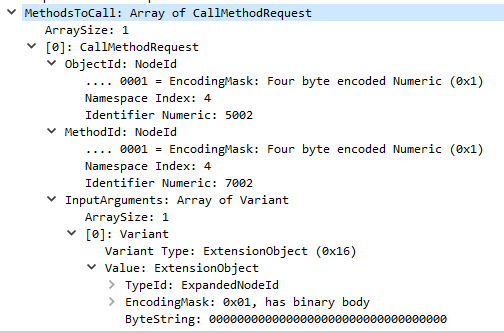
\includegraphics[width=(\textwidth/2)]{Bild/StartScabWireshark.PNG}
    \caption{StartScan über Wireshark}
    \label{fig:StartScanueberWireshark}
\end{figure}

Der OpcUa-Service ist ein \dq Encodeable Object\dq  mit dem TypeId \dq ExpandedNodeId\dq . Es wird eine \dq CallRequest\dq  ausgeführt, die einen \dq RequestHeader\dq  und eine \dq MethodToCall\dq -Liste enthält. Die Liste hat eine Größe von 1 und enthält einen \dq CallMethodRequest\dq . Dieser hat eine \dq ObjectId\dq  und eine \dq MethodId\dq , die jeweils durch eine \dq NodeId\dq  dargestellt werden.\\

Der \dq CallMethodRequest\dq  enthält auch eine \dq InputArguments\dq -Liste mit einer Größe von 1, die einen \dq Variant\dq  enthält. Dieser hat den Variant-Typ \dq ExtensionObject\dq  und einen \dq Value\dq , der wiederum ein \dq ExtensionObject\dq  ist. Dieses hat eine TypeId und einen ByteString mit einer Länge von 40 Bytes, der alle Nullen enthält.\\

Wie kann man die Methode aufrufen?

Ein Methodenaufruf ermöglicht es, Eingabe- und Ausgabeargumente an/von einer Methode zu übergeben. Diese Argumente werden durch Eigenschaften der Methode definiert.\\

Der Aufruf benötigt die NodeId der jeweiligen Methode. Die Node Ids können aus dem UAExpert oder aus dem Wireshark gelesen werden.
\begin{lstlisting}[style=JavaScript, caption={Methodenaufruf StartScan}]
const methodToCall: CallMethodRequestLike = {
    methodId: (`ns=${this.nsRfu};i=7002`),
    objectId: (`ns=${this.nsRfu};i=5002`),
    inputArguments: [
        {
        dataType: DataType.ExtensionObject,
        value: scanSettingsObj
        }
    ]
};

// Call method, passing ScanSettings as input argument
    await this.session.call(methodToCall,(err,results) => {
        if (err) {
            console.log(err);
        } else {
            console.log(results);
        }
    });
\end{lstlisting}

Der Code verwendet die OPC UA-Bibliothek und ruft eine Methode auf einem Remote-Server auf.\\

Der Code definiert zuerst ein Objekt namens \dq methodToCall\dq  mit den Eigenschaften \dq methodId\dq , \dq objectId\dq  und \dq inputArguments\dq . \dq methodId\dq  und \dq objectId\dq  definieren die OPC UA-Methoden-ID und Objekt-ID, die aufgerufen werden sollen. \dq inputArguments\dq  definiert die Eingabeargumente, die an die aufgerufene Methode übergeben werden sollen.\\

Dann wird die Methode mit \dq session.call\dq  aufgerufen und die Eingabeargumente werden übergeben. Das Ergebnis des Methodenaufrufs wird in einer Rückruffunktion verarbeitet, wobei eventuelle Fehler in der Konsole ausgegeben werden und das Ergebnis des Methodenaufrufs angezeigt wird.

\subsection*{Konstruieren eines Extensionobject}

Das ExtensionObject ist das Input-Argument für die StartScan-Methode. Es enthält die gleichen Parameter wie diejenigen, die auch in UAExpert eingegeben werden müssen, um den Scan zu starten. Im Python-Code \ref{StartScanPython} sind diese Parameter enthalten.\\

Was ist ein ExtensionObject?

Ein ExtensionObject ist ein Behälter für strukturierte Datentypen, die nicht als einer der anderen eingebauten Datentypen codiert werden können. Das ExtensionObject enthält einen komplexen Wert, der als Sequenz von Bytes oder als XML-Element serialisiert ist. Es enthält auch einen Identifier, der angibt, welche Daten es enthält und wie sie codiert sind.\\

Strukturierte Datentypen werden im Server-Adressraum als Unterarten des Strukturdatentyps dargestellt. Die verfügbaren Datenkodierungen für jeden Strukturierten Datentyp werden als DataTypeEncoding-Objekt im Server AddressSpace dargestellt. Die NodeId für das DataTypeEncoding-Objekt ist die Kennung, die im ExtensionObject gespeichert ist.\\

Es werden namensraumqualifizierte numerische NodeIds für alle definierten DataTypeEncoding-Objekte verwenden. Dies minimiert den Overhead, der durch das Verpacken von strukturierten Datentypwerten in ein ExtensionObject eingeführt wird.\\

Die OPCUA-Bibliothek enthält einen Test, der auch die \dq ScanSettings\dq  in ein \dq ExtensionObject\dq  kodiert. Die Eingaben, die zur Erstellung des \dq ExtensionObject\dq  verwendet werden, sind dieselben wie diejenigen, die in UA Expert eingegeben werden müssen, um den Scan zu starten.\\

\begin{lstlisting}[style=JavaScript, caption={ExtensionObject ScanSettings Test}]
enum LocationTypeEnumeration {
    NMEA = 0, // An NMEA string representing a coordinate as defined in 9.1.2.
    LOCAL = 2, // A local coordinate as defined in 9.3.4
    WGS84 = 4, // A lat / lon / alt coordinate as defined in 9.3.16
    NAME = 5 // A name for a location as defined in 9.1.1
}
interface ScanSettings extends ExtensionObject {
    duration: number;
    cycles: number;
    dataAvailable: boolean;
    locationType?: LocationTypeEnumeration;
}
const scanSettingsDataTypeNode = addressSpace.findDataType("ScanSettings", nsAutoId)!;

const settings = addressSpace.constructExtensionObject(scanSettingsDataTypeNode, {}) as ScanSettings;
\end{lstlisting}

Der Code definiert eine Enumeration namens \dq LocationTypeEnumeration\dq , die verschiedene Arten von Ortsangaben für einen Scan darstellt, einschließlich Koordinaten in verschiedenen Formaten und einem Ortsnamen.\\

Dann wird eine Schnittstelle namens \dq ScanSettings\dq  erstellt, die das \dq ExtensionObject\dq  erweitert. Diese Schnittstelle enthält einige Eigenschaften wie \dq duration\dq  (Dauer), \dq cycles\dq  (Zyklen), \dq dataAvailable\dq  (Daten verfügbar) und optional \dq locationType\dq  (Ortsangabe-Typ).\\

Das \dq ExtensionObject\dq  ist ein Container für strukturierte Datentypen, die nicht als einer der anderen eingebauten Datentypen kodiert werden können. Der Code verwendet die \dq constructExtensionObject\dq -Methode, um ein \dq ExtensionObject\dq  vom Typ \dq ScanSettings\dq  zu erstellen.\\

Beim Versuch, den Code auszuführen, treten Fehler auf, da es nicht möglich ist, die NodeId für das \dq ExtensionObject\dq  mit der Methode \dq findDataType\dq  zu finden.\\

Es ist jedoch möglich, die NodeId des jeweiligen UAExpert auszulesen oder sie im Wireshark zu suchen und diese dann hardcoded in den Code einzutragen.\\

\begin{lstlisting}[style=JavaScript, caption={ScanSettingsObj}]
const scanSettingsParams = {
    duration : aduration,
    cycles : acycles,
    dataAvailable : adataAvailable,
    locationType: 0
}
// NodeID for InputArguments struct type (inherits from ScanSettings)
const nodeID = new NodeId(NodeIdType.NUMERIC, 3010, 3);

// Create ExtensionObject for InputArguments
const scanSettingsObj = await this.session.constructExtensionObject(nodeID, scanSettingsParams)
\end{lstlisting}

Zunächst wird eine NodeId-Objekt erstellt, das die numerische ID des Typs der Struktur InputArguments enthält, die von der ScanSettings-Struktur erbt.\\

Das NodeId-Objekt wird mit Hilfe des new Schlüsselwortes und des NodeIdType.NUMERIC Enumerators erstellt. Der erste Parameter gibt den Typ der NodeID an und der zweite und dritte Parameter geben die numerischen Werte der NodeID an.\\

Dann wird die constructExtensionObject-Methode der Session-Klasse aufgerufen, um das ExtensionObject-Objekt zu erstellen. Diese Methode nimmt zwei Parameter entgegen, nämlich die NodeId und das scanSettingsParams-Objekt, das die Einstellungen des Scans enthält.\\

Das Schlüsselwort await wird verwendet, um die asynchrone Ausführung des Codes zu ermöglichen und sicherzustellen, dass das scanSettingsObj-Objekt vollständig erstellt wird, bevor es verwendet wird. Das resultierende Objekt ist das ExtensionObject, das die Einstellungen des Scans im System enthält.\\

Das erstellte ExtensionObject kann als inputArgument in den MethodenRequest aufgenommen werden und den Scan zustarten.

\section{LastScanData ReadMethode}
Was soll die Methode zurückgegeben?

Die Methode gibt die Daten des letzten Scans zurück. Diese beinhalten die TagId eines möglichen RFID-Tags, der vom RFID-Scanner gescannt wird. Um auf die Daten zuzugreifen, muss zuvor die StartScan-Methode aufgerufen werden und es müssen Daten empfangen werden.\\

Was ist ein Session read?

Um auf die Knoten LastScanData zuzugreifen, ist keine Methode mit einem MethodRequest erforderlich, sondern eine Read-Methode.\\

Dieser Service wird verwendet, um ein oder mehrere Attribute von einem oder mehreren Knoten zu lesen. Bei konstruierten Attributwerten, deren Elemente indexiert sind, z.B. ein Array, ermöglicht dieser Service den Clients das Lesen des gesamten Satzes indexierter Werte als Composite, das Lesen einzelner Elemente oder das Lesen von Bereichen von Elementen des Composite.\\

Der Parameter \dq maxAge \dq wird verwendet, um den Server anzuweisen, den Wert aus der zugrunde liegenden Datenquelle, wie z.B. einem Gerät, abzurufen, wenn dessen Kopie der Daten älter ist als das, was der "maxAge" angibt. Wenn der Server das angeforderte maximale Alter nicht erfüllen kann, gibt er seinen "besten Versuchswert" zurück, anstatt die Anfrage abzulehnen. MaxAge wird beim erstellen des Client festgelegt.\\

\begin{lstlisting}[style=JavaScript, caption={ScanSettingsObj}]
const nodeToRead = {
    nodeId:      `ns=${this.nsRfuId};i=6023`,
    attributeId: AttributeIds.Value
};
const lastScanData = await this.session.read(nodeToRead);
return lastScanData.value.value;
\end{lstlisting}
Der Code definiert zunächst eine Konstante namens \dq nodeToRead\dq , die ein Objekt-Literal enthält. Dieses Objekt hat zwei Eigenschaften: \dq nodeId\dq  und \dq attributeId\dq . Die \dq nodeId\dq  Eigenschaft enthält eine Zeichenkette, die die Node-ID im OPC-UA-Server angibt, von der Daten gelesen werden sollen. Die \dq attributeId\dq  Eigenschaft gibt an, welches Attribut des Knotens (Node) gelesen werden soll. In diesem Fall soll das Attribut \dq Value\dq  gelesen werden, was bedeutet, dass der tatsächliche Wert der Node zurückgegeben wird.\\

Anschließend wird eine weitere Konstante namens \dq lastScanData\dq  definiert, die auf das Ergebnis einer asynchronen Operation wartet. Diese asynchrone Operation wird mit \dq await\dq  und \dq this.session.read(nodeToRead)\dq  ausgeführt, wobei \dq this.session\dq  eine Referenz auf eine Verbindungssitzung zum OPC-UA-Server ist. Der Befehl \dq read\dq  liest die Daten von der angegebenen Node-ID im Server.\\

Schließlich wird der Wert der Eigenschaft \dq value\dq  im Objekt \dq lastScanData\dq  zurückgegeben, der den tatsächlichen Wert der gelesenen Node enthält. Die Node wurde aus einer Aufnahme von Wireshark gelesen als mit dem UaExpert LastScandata aufgerufen wird.

\section{ReadTag CallMethode}

Die ReadTag-Methode wird verwendet, um die Daten des Tags mit der entsprechenden ID auszulesen.

Auf dem RFID Tag können ByteString gespeichert werden. Die mit der Write Methode ausgelesen werden.

Wie das Inputargument aufgebaut wird, erdeutet sich aus dem UAExpert und aus dem Wireshark Aufnahme des UaExpert, wenn dieser die ReadTag Methode aufruft. 

\begin{figure}[H]
    \centering
    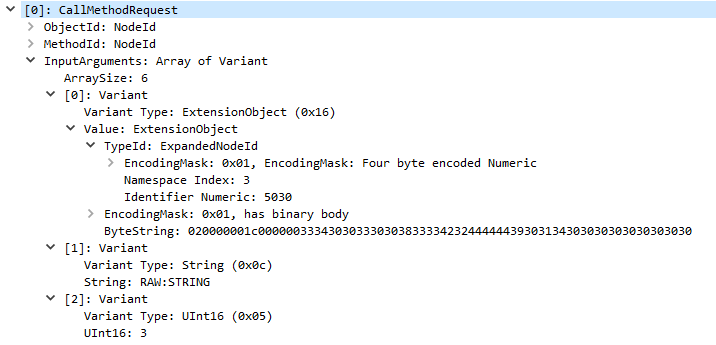
\includegraphics[width=(\textwidth/2)]{Bild/WriteTagWireshark.PNG}
    \caption{StartScan über Wireshark}
    \label{fig:WriteueberWireshark}
\end{figure}

\begin{lstlisting}[style=JavaScript, caption={ReadTag Methode}]
async ReadTag(tagId : string, codetype : string, region : number, offset : number, length : number){

    const identiferParams = {
        string: tagId	
    }

    const identifierId = new NodeId (NodeIdType.NUMERIC, 3020, 3);
    const identifierObj = await this.session!.constructExtensionObject(identifierId, identiferParams);
    
    const methodToCall : CallMethodRequestLike = {
        methodId : (`ns=${this.nsRfuId};i=7004`),
        objectId : (`ns=${this.nsRfuId};i=5002`),
        inputArguments : [{
            dataType : DataType.ExtensionObject,
            value : identifierObj
        },
        {
            dataType : DataType.String,
            value : codetype
        },
        {
            dataType : DataType.UInt16,
            value : region
        },
        {
            dataType : DataType.UInt32,
            value : offset
        },
        {
            dataType : DataType.UInt32,
            value : length
        },
        {
            dataType : DataType.String,
            value : ""
        }
        ]
    };
    this.session!.call(methodToCall,(err,results) => {
            if (err) {
                console.log(err);
            } else {
                console.log("ReadTag Result: ",results);
            }
        });
}
\end{lstlisting}

Dieser Code definiert eine asynchrone Funktion ReadTag, die fünf Argumente erwartet: tagId (ein String), codetype (ein String), region (eine Zahl), offset (eine Zahl) und length (eine Zahl). Die Funktion ruft eine Methode in einem OPC UA-Server auf, um den Wert eines Tags auszulesen.\\

In der Funktion wird zuerst ein Objekt identifierParams erstellt, das einen Parameter string enthält, der den Wert von tagId enthält. Dann wird ein neues NodeId-Objekt erstellt, das die numerische ID 3020 und den Typ 3 enthält. Diese NodeId-Instanz wird verwendet, um ein Extension-Objekt zu erstellen, das das identifierParams-Objekt als Parameter enthält. Das Ergebnis wird in der Variable identifierObj gespeichert.\\

Dann wird ein methodToCall-Objekt erstellt, das die Methoden-ID und Objekt-ID für den OPC UA-Server enthält. Die Eingabe-Argumente für die aufzurufende Methode werden ebenfalls in diesem Objekt definiert. Das identifierObj-Objekt wird als Extension-Objekt für das erste Argument verwendet, während die restlichen Argumente vom Typ DataType.String, DataType.UInt16, DataType.UInt32 und DataType.String sind.\\

Schließlich wird die call-Methode der session-Instanz aufgerufen, um die Methode auf dem OPC UA-Server auszuführen. Wenn ein Fehler auftritt, wird er in der Konsole ausgegeben. Andernfalls wird das Ergebnis der Methode in der Konsole ausgegeben.\\

Es ist zu beachten, dass die call-Methode asynchron ist und ein Callback-Funktion als zweites Argument erwartet, die aufgerufen wird, wenn die Methode auf dem Server ausgeführt wurde und ein Ergebnis zurückgegeben wurde. In diesem Fall wird der Callback verwendet, um das Ergebnis der Methode auszugeben.\\



\section{EventRegistration}
%Was soll die methode machen?

Die Methode registriert das Event RfidScanResult und gibt dieses in der Connsole aus.

Ein OPCUA Event zu registriert und zu abonieren ist wie Datenänderungen, aber anstatt einen Datenänderungsfilter zu verwenden wird ein Eventfilter verwendet.\\

%Was ist ein Events?

Events repräsentieren spezifische Ereignisse. Event-Benachrichtigungen melden das Auftreten eines Events. Objekte und Ansichten können genutzt werden, um sich für Events anzumelden. Das EventNotifier-Attribut dieser Knoten identifiziert, ob der Knoten das Abonnieren von Events erlaubt. Clients melden sich bei solchen Knoten an, um Benachrichtigungen über das Auftreten von Events zu erhalten.\\

Event-Abonnements verwenden Monitoring- und Abonnement-Dienste, um sich für die Event-Benachrichtigungen eines Knotens anzumelden.\\

Jeder OPC UA-Server, der Eventing unterstützt, muss mindestens einen Knoten als EventNotifier bereitstellen. Das Serverobjekt wird hierfür verwendet. Events, die vom Server generiert werden, stehen über dieses Serverobjekt zur Verfügung.\\

%Was ist ein Eventfilter?

Der EventFilter ermöglicht die Filterung und Auswahl von Event-Abonnements.
Wenn eine Event-Benachrichtigung dem Filter entspricht, wird sie an den Client gesendet. Der Event-Filter gibt an, welche Felder in der Event-Benachrichtigung
enthalten sein sollen und welche Event-Typen unterstützt werden. Der SimpleAttributeOperand Struktur wird verwendet, um die Event-Attribute auszuwählen, die zurückgegeben werden sollen.  Der EventFilter prüft auch auf strukturelle Fehler beim Erstellen oder Aktualisieren des
Filters.\\

%Wie ist das Vorgehen?

Es ist möglich die EventRegistration Methode über den UAExpert auszuführen. Bei der beobachtung mit Wireshark muss beachtet werden welche Paket relevant sind für die Anforderung an die Methode.

%Wie wird es im UAExpert gemacht?

%Was sagt Wireshark?

Die relevantesten Pakete sind die Erstellung einer Subscription und die Erstellung eines MonitoringItem.

%Was ist eine Subscription?

Eine Subscription wird dazu genutzt Nachrichten oder Benachrichtigung an
den Client zusenden. Subscriptions haben MonitoredItem die Benachrichtigungen generieren, die an den Client gesendet werden. Die Subscriptiom haben auch eine Veröentlichungsrate und eine Keep-alive -Zähler, der angibt,
wie viele Zyklen ohne Benachrichtigung es gegeben hat. Wenn der maximale
keep-alive-Zähler errechtj ist, wird eine Nachricht gesendet, um den Client
darüber zu informieren, dass die Subscription noch aktiv ist.\\
Nach der Erstellung der Subscription startet der Server den Veröentlichungstimer und startet ihn neu, wenn er abläuft. Wenn der Timer abläuft,
ohne dass vom Client eine Subscription-Service-Request empfangen wurde
und die Anzahl der Subscriptionlebensdauer abgelaufen ist, geht die Subscription davon aus, dass der Client nicht mehr vorhanden ist und wird beendet.\\

%Keep alive Count hat er was damit zu tun wann die Subcription geschlossen wird?
Wenn \dq keep-alive \dq den Wert erreicht, der für die Lebensdauer einer Subscription basierend auf dem MaxKeepAliveCount-Parameter im CreateSubscriptionService berechnet wird, wird die Subscription geschlossen.
Das Attribut gibt die Priorität des Abonnements an. Wenn mehrere
Abonnements Benachrichtigungen senden müssen, wird der Server die Veröentlichungsanfrage an das Abonnement mit der höchsten Priorität weiterleiten. Wenn die Keep-Alive-Zeit abläuft, hat das Abonnement Vorrang, um
das Ablaufen zu verhindern. Wenn ein Client keine besonderen Prioritätseinstellungen benötigt, sollte der Wert auf Null gesetzt werden.\\

%Was ist die CreateSubscription?
\begin{lstlisting}[style=JavaScript, caption={SubscriptionForEventRegistration}]
async SubscriptionForEventRegistration(){
    // step 5: install a subscription and install a monitored item for 10 seconds
    const subscription = ClientSubscription.create(this.session!, {
        requestedPublishingInterval: 500,
        requestedLifetimeCount: 2400,
        requestedMaxKeepAliveCount: 10,
        maxNotificationsPerPublish: 65535,
        publishingEnabled: true,
        priority: 0                   //the priority of a subscription, determining the order in which Publish requests are dequeued and processed by the server
    });

    subscription
        .on("started", function () {
        console.log(
            "subscription started for 2 seconds - subscriptionId=",
            subscription.subscriptionId
        );
        })
        .on("keepalive", function () {
        console.log("keepalive");
        })
        .on("terminated", function () {
        console.log("terminated");
        });
    return subscription;
}
\end{lstlisting}

Der Code implementiert eine asynchrone Funktion namens "SubscriptionForEventRegistration", die eine Subscription erstellt, um überwachte Elemente (monitored items) zu empfangen.\\

Es wird eine Subscription mit bestimmten Einstellungen erstellt, einschließlich des gewünschten Veröffentlichungsintervalls, der Anzahl der erwarteten Lebensdauerereignisse, der maximalen Anzahl von Keepalive-Ereignissen, die empfangen werden sollen, der maximalen Anzahl von Benachrichtigungen, die pro Veröffentlichung empfangen werden sollen, und der Priorität der Subscription.\\

Das "subscription" Objekt wird durch Aufruf der "create" Methode auf einem "ClientSubscription" Objekt erstellt und zurückgegeben, sobald es erfolgreich initialisiert wurde.\\

Die Ereignisse "started", "keepalive" und "terminated" werden überwacht, um den Status der Subscription zu überwachen. Sobald die Subscription gestartet ist, wird die subscriptionId ausgegeben. Bei Keepalive-Ereignissen wird die Ausgabe "keepalive" generiert, um anzuzeigen, dass die Verbindung aktiv bleibt. Wenn die Subscription terminiert wird, wird die Ausgabe "terminated" generiert.\\

%Was ist ein Monitoring Item?

Die Monitoring Items werden genutzt um über eine Subscription daten zu
empfangen. Es wird initaliesiert mit dem \dq sampling interval \dq , dem monttoring mode, dem Filter und den \dq queue parameter \dq . Wenn der Client
nur Ereignisse abonniert, wird eine \dq sampling interval \dq von 0 deniert. Eine
negative Zahl fordert das Standard-Abtastintervall an.
Der Client kann auch eine Abtastfrequenz von 0 angeben, um den schnellstmöglichen Abtastintervall zu verwenden. Es wird erwartet, dass Server nur
eine begrenzte Anzahl von Abtastfrequenzen unterstützen, um ihren Betrieb
zu optimieren. Wenn der vom Client angeforderte genaue Intervall nicht unterstützt wird, weist der Server dem MonitoredItem das am besten geeignete
Intervall zu und gibt dieses dem Client zurück. Der Server Capability Object
identißziert die unterstützten Abtastfrequenzen.\\
Der Server kann Daten unterstützen, die auf einem Abtastmodell basieren oder auf einem Ausnahme-Modell generiert werden. Das schnellste
unterstützte Abtastintervall kann gleich 0 sein, was bedeutet, dass das Datenobjekt ausnahmsbasiert ist und keine periodische Abtastung erfordert.\\
Jedes Mal, wenn ein MonitoredItem abgetastet wird, bewertet der Server
die Probe mithilfe des für das MonitoredItem defnierten Filters. Der Filterparameter defniert die Kriterien, die der Server verwendet, um zu bestimmen, ob eine Benachrichtigung für die Probe generiert werden soll. Der Typ
des Filters hängt vom Typ des überwachten Elements ab. Beispielsweise werden DataChangeFilter und AggregateFilter verwendet, wenn Variablenwerte
überwacht werden, und EventFilter wird verwendet, wenn Ereignisse überwacht werden. Die Abtastung und Bewertung einschlieÿlich der Verwendung
von Filtern werden in diesem Standard beschrieben. Weitere Filter können
in anderen Teilen dieser Reihe von Standards deniert werden.

\begin{lstlisting}[style=JavaScript, caption={MonitoredItemAddToSubscription}]
async MonitoredItemAddToSubscription(subscription : ClientSubscription){
    const fields = [
        `${this.nsAutoId}:ScanResult`
    ];

    const eventFilter = constructEventFilter(fields);

    const parameters: MonitoringParametersOptions = {
        samplingInterval: 0,
        discardOldest: true,
        queueSize: 4294967295,
        filter: eventFilter
    };

    const itemToMonitor = {
        nodeId: "ns=0;i=2253",
        attributeId: AttributeIds.EventNotifier
    };


    const monitoredItem = ClientMonitoredItem.create(
        subscription,
        itemToMonitor,
        parameters,
        TimestampsToReturn.Both
    );
    ...
    
    monitoredItem.on("changed", (dataValue: Variant[]) => {
        console.log(dataValue[0].value);
        console.log(dataValue[0].value[0].scanData.byteString);
    });
}
\end{lstlisting}

Die Funktion \dq MonitoredItemAddToSubscription \dq erstellt einen überwachten OPC-UA-Client-Parameter namens "monitoredItem". Ein überwachter Parameter ermöglicht es einem OPC-UA-Client, bestimmte Ereignisse oder Datenänderungen in einem OPC-UA-Server zu überwachen.\\

Der Code definiert zunächst ein Array mit einem Element, das den vollqualifizierten Namen eines Ereignisses (ScanResult) enthält, das der Client überwachen möchte.\\

Dann wird eine Eventfilterkonfiguration aus diesem Array erstellt.\\

Als nächstes werden Überwachungsparameter definiert, einschließlich der Sampling-Intervallzeit, der Verwerfung ältester Proben, der maximale Queue-Größe und der Eventfilterkonfiguration.\\

Schließlich wird ein OPC-UA-Objekt mit dem zu überwachenden Knoten- und Attribut-ID, den Überwachungsparametern und der Anforderung zur Rückgabe des Zeitstempels erstellt.\\

Nach der Erstellung des überwachten OPC-UA-Clients "monitoredItem" wird ein Ereignis-Listener hinzugefügt, der auf Änderungen dieses Ereignisses reagiert. Wenn sich das Ereignis "ScanResult" ändert, werden die Daten des Ereignisses in der Variablen "dataValue" gespeichert und über die Konsole ausgegeben.\\

Die ersten beiden Ausgaben geben den Wert des ersten Elements des "dataValue"-Arrays aus. Die dritte Ausgabe greift auf das byteString-Attribut dieses Objekts zu und gibt es auf der Konsole aus. Dies kann zur weiteren Verarbeitung oder Anzeige der gescannten Daten verwendet werden.\\


\section{BrowsePath}